\renewcommand*{\arraystretch}{1.1}

\subsection*{Interactive / complex / 3}
\label{section:interactive-complex-read-03}

% change \emph{} to use sans-serif font
\let\oldemph\emph
\renewcommand{\emph}[1]{{\footnotesize \sf #1}}

\renewcommand{\currentQueryCard}{3}
\marginpar{
	\raggedleft
	\vspace{0.22ex}

	\queryRefCard{interactive-complex-read-01}{IC}{1}\\
	\queryRefCard{interactive-complex-read-02}{IC}{2}\\
	\queryRefCard{interactive-complex-read-03}{IC}{3}\\
	\queryRefCard{interactive-complex-read-04}{IC}{4}\\
	\queryRefCard{interactive-complex-read-05}{IC}{5}\\
	\queryRefCard{interactive-complex-read-06}{IC}{6}\\
	\queryRefCard{interactive-complex-read-07}{IC}{7}\\
	\queryRefCard{interactive-complex-read-08}{IC}{8}\\
	\queryRefCard{interactive-complex-read-09}{IC}{9}\\
	\queryRefCard{interactive-complex-read-10}{IC}{10}\\
	\queryRefCard{interactive-complex-read-11}{IC}{11}\\
	\queryRefCard{interactive-complex-read-12}{IC}{12}\\
	\queryRefCard{interactive-complex-read-13}{IC}{13}\\
	\queryRefCard{interactive-complex-read-14}{IC}{14}\\
}


\noindent\begin{tabularx}{\queryCardWidth}{|>{\queryPropertyCell}p{\queryPropertyCellWidth}|X|}
	\hline
	query & Interactive / complex / 3 \\ \hline
%
	title & Friends and friends of friends that have been to countries X and Y \\ \hline
%
	pattern & \centering 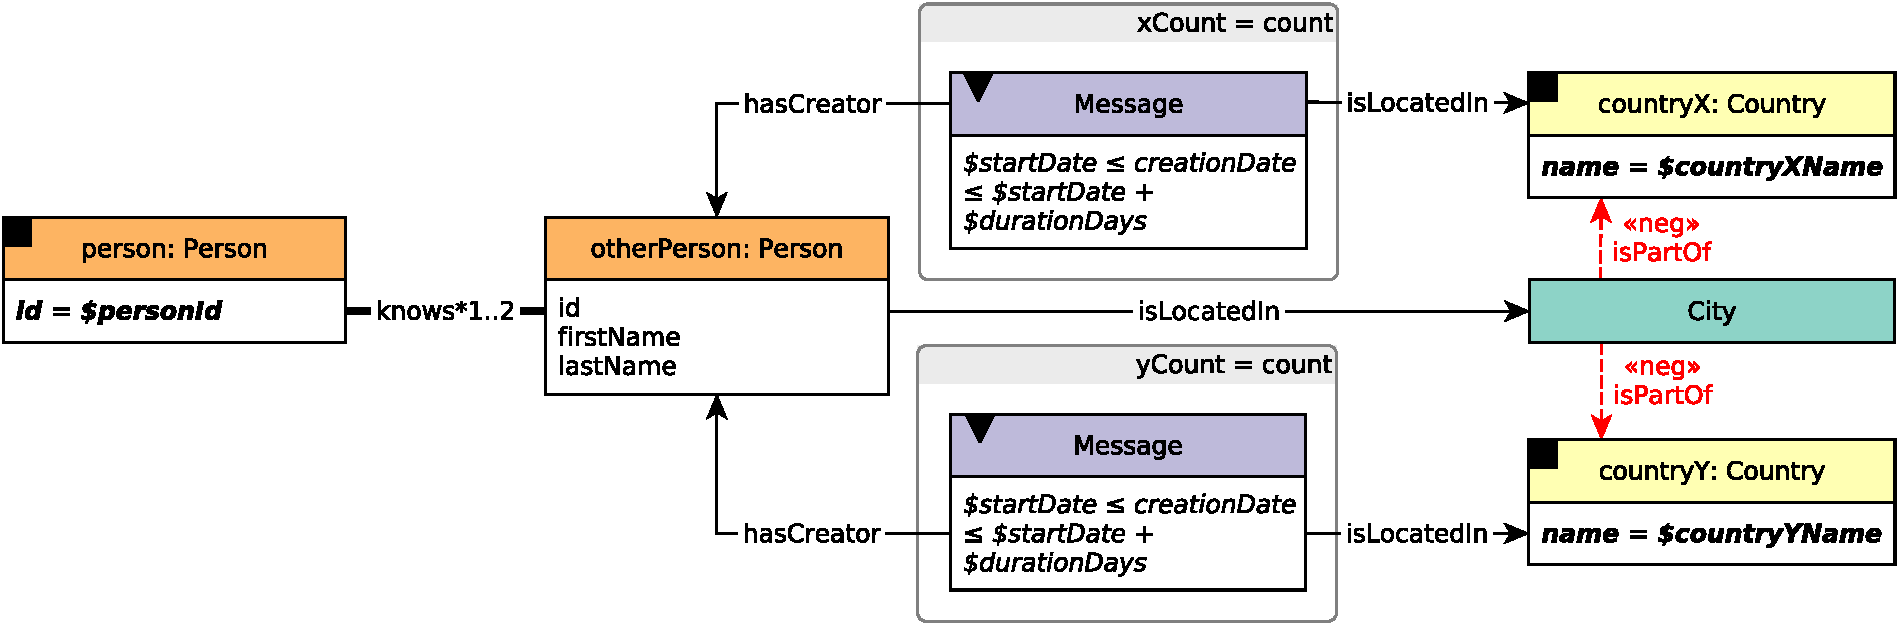
\includegraphics[scale=\patternscale,margin=0cm .2cm]{patterns/interactive-complex-read-03} \tabularnewline \hline
%
	desc. & Given a start \emph{Person}, find \emph{Persons} that are their friends
and friends of friends (excluding start \emph{Person}) that have made
\emph{Posts} / \emph{Comments} in both of the given \emph{Countries},
\texttt{CountryX} and \texttt{CountryY}, within a given period. Only
\emph{Persons} that are foreign to \emph{Countries} \texttt{CountryX}
and \texttt{CountryY} are considered, that is \emph{Persons} whose
location is neither \texttt{CountryX} nor \texttt{CountryY}.
 \\ \hline
%
	
		params &
		\innerCardVSpace{\begin{tabularx}{\attributeCardWidth}{|>{\paramNumberCell}c|>{\varNameCell}M|>{\typeCell}m{\typeWidth}|Y|} \hline
		$\mathsf{1}$ & Person.id
 & ID
 & \texttt{personId}
 \\ \hline
		$\mathsf{2}$ & CountryX.name
 & String
 & \texttt{countryXName}
 \\ \hline
		$\mathsf{3}$ & CountryY.name
 & String
 & \texttt{countryYName}
 \\ \hline
		$\mathsf{4}$ & startDate
 & Date
 & \texttt{startDate} -- Beginning of requested period
 \\ \hline
		$\mathsf{5}$ & duration
 & 32-bit Integer
 & \texttt{durationDays} -- Duration of requested period, in days the
interval \texttt{{[}startDate,\ startDate\ +\ duration)} is closed-open
 \\ \hline
		\end{tabularx}}\innerCardVSpace \\ \hline
	
%
	
		result &
		\innerCardVSpace{\begin{tabularx}{\attributeCardWidth}{|>{\resultNumberCell}c|>{\varNameCell}M|>{\typeCell}m{\typeWidth}|>{\resultOriginCell}c|Y|} \hline
		$\mathsf{1}$ & Person.id & ID & R &
				\texttt{personId}
 \\ \hline
		$\mathsf{2}$ & Person.firstName & String & R &
				\texttt{personFirstName}
 \\ \hline
		$\mathsf{3}$ & Person.lastName & String & R &
				\texttt{personLastName}
 \\ \hline
		$\mathsf{4}$ & xCount & 32-bit Integer & A &
				\texttt{xCount} -- Number of \emph{Messages} from \emph{Country}
\texttt{CountryX} created by the \emph{Person} within the given time
 \\ \hline
		$\mathsf{5}$ & yCount & 32-bit Integer & A &
				\texttt{yCount} -- Number of \emph{Messages} from \emph{Country}
\texttt{CountryY} created by the \emph{Person} within the given time
 \\ \hline
		$\mathsf{6}$ & count & 32-bit Integer & A &
				\texttt{count} = \texttt{xCount} + \texttt{yCount}
 \\ \hline
		\end{tabularx}}\innerCardVSpace \\ \hline
	
%
	
		sort		&
		\innerCardVSpace{\begin{tabularx}{\attributeCardWidth}{|>{\sortNumberCell}c|>{\varNameCell}M|>{\directionCell}c|Y|} \hline
		$\mathsf{1}$ & xCount
 & $\desc
$ &  \\ \hline
		$\mathsf{2}$ & Person.id
 & $\asc
$ &  \\ \hline
		\end{tabularx}}\innerCardVSpace \\ \hline
	%
	limit & 20 \\ \hline
	%
	CPs &
	\multicolumn{1}{>{\raggedright}l|}{
		\chokePoint{2.1}, 
		\chokePoint{3.1}, 
		\chokePoint{5.1}, 
		\chokePoint{8.2}, 
		\chokePoint{8.5}
		} \\ \hline
	%
	relevance &
		\footnotesize This query looks for paths of length two and three, starting from a *Person*, going to friends or friends of friends, and then moving to *Messages*. This query tests the ability of the query optimizer to select the most efficient join ordering, which will depend on the cardinalities of the intermediate results. Many friends of friends can be duplicate, then it is expected to eliminate duplicates and those people prior to access the *Post* and *Comments*, as well as eliminate those friends from *Countries* `CountryX` and `CountryY`, as the size of the intermediate results can be severely affected. A possible structural optimization could be to materialize the number of *Posts* and *Comments* created by a *Person*, and progressively filter those people that could not even fall in the top 20 even having all their posts in the *Countries* `CountryX` and `CountryY`.
 \\ \hline%
\end{tabularx}
\queryCardVSpace

% change \emph back to the old one
\let\emph\oldemph